%%%%%%%%%%%%  Generated using docx2latex.com  %%%%%%%%%%%%%%

%%%%%%%%%%%%  v2.0.0-beta  %%%%%%%%%%%%%%

\documentclass[12pt]{article}
\usepackage{amsmath}
\usepackage{latexsym}
\usepackage{amsfonts}
\usepackage[normalem]{ulem}
\usepackage{array}
\usepackage{amssymb}
\usepackage{graphicx}
\usepackage[backend=biber,
style=numeric,
sorting=none,
isbn=false,
doi=false,
url=false,
]{biblatex}\addbibresource{bibliography.bib}

\usepackage{subfig}
\usepackage{wrapfig}
\usepackage{wasysym}
\usepackage{enumitem}
\usepackage{adjustbox}
\usepackage{ragged2e}
\usepackage[svgnames,table]{xcolor}
\usepackage{tikz}
\usepackage{longtable}
\usepackage{changepage}
\usepackage{setspace}
\usepackage{hhline}
\usepackage{multicol}
\usepackage{tabto}
\usepackage{float}
\usepackage{multirow}
\usepackage{makecell}
\usepackage{fancyhdr}
\usepackage{pgf}
\usepackage{pgfpages}
\usepackage[toc,page]{appendix}
\usepackage[hidelinks]{hyperref}
\usetikzlibrary{shapes.symbols,shapes.geometric,shadows,arrows.meta}
\tikzset{>={Latex[width=1.5mm,length=2mm]}}
\usepackage{flowchart}\usepackage[paperheight=11.69in,paperwidth=8.27in,left=1.0in,right=1.0in,top=1.0in,bottom=1.0in,headheight=1in]{geometry}
\usepackage[utf8]{inputenc}
\usepackage[T1]{fontenc}
\TabPositions{0.5in,1.0in,1.5in,2.0in,2.5in,3.0in,3.5in,4.0in,4.5in,5.0in,5.5in,6.0in,}

\urlstyle{same}


 %%%%%%%%%%%%  Set Depths for Sections  %%%%%%%%%%%%%%

% 1) Section
% 1.1) SubSection
% 1.1.1) SubSubSection
% 1.1.1.1) Paragraph
% 1.1.1.1.1) Subparagraph


\setcounter{tocdepth}{5}
\setcounter{secnumdepth}{5}


 %%%%%%%%%%%%  Set Depths for Nested Lists created by \begin{enumerate}  %%%%%%%%%%%%%%


\setlistdepth{9}
\renewlist{enumerate}{enumerate}{9}
		\setlist[enumerate,1]{label=\arabic*)}
		\setlist[enumerate,2]{label=\alph*)}
		\setlist[enumerate,3]{label=(\roman*)}
		\setlist[enumerate,4]{label=(\arabic*)}
		\setlist[enumerate,5]{label=(\Alph*)}
		\setlist[enumerate,6]{label=(\Roman*)}
		\setlist[enumerate,7]{label=\arabic*}
		\setlist[enumerate,8]{label=\alph*}
		\setlist[enumerate,9]{label=\roman*}

\renewlist{itemize}{itemize}{9}
		\setlist[itemize]{label=$\cdot$}
		\setlist[itemize,1]{label=\textbullet}
		\setlist[itemize,2]{label=$\circ$}
		\setlist[itemize,3]{label=$\ast$}
		\setlist[itemize,4]{label=$\dagger$}
		\setlist[itemize,5]{label=$\triangleright$}
		\setlist[itemize,6]{label=$\bigstar$}
		\setlist[itemize,7]{label=$\blacklozenge$}
		\setlist[itemize,8]{label=$\prime$}



 %%%%%%%%%%%%  Header here  %%%%%%%%%%%%%%


\pagestyle{fancy}
\fancyhf{}
\chead{\fontsize{10pt}{12.0pt}\selectfont New Approach to SCM (Supply Chain Management) using Blockchain}
\rfoot{\fontsize{10pt}{12.0pt}\selectfont Department of TE Computer Engineering, DYPIET, Pimpri}
\rhead{\thepage}
\renewcommand{\headrulewidth}{0pt}
\setlength{\topsep}{0pt}\setlength{\parindent}{0pt}

 %%%%%%%%%%%%  This sets linespacing (verticle gap between Lines) Default=1 %%%%%%%%%%%%%%


\renewcommand{\arraystretch}{1.3}

\pgfpagesdeclarelayout{boxed}
{
  \edef\pgfpageoptionborder{0pt}
}
{
  \pgfpagesphysicalpageoptions
  {%
    logical pages=1,%
  }
  \pgfpageslogicalpageoptions{1}
  {
    border code=\pgfsetlinewidth{2pt}\pgfstroke,%
    border shrink=\pgfpageoptionborder,%
    resized width=.95\pgfphysicalwidth,%
    resized height=.95\pgfphysicalheight,%
    center=\pgfpoint{.5\pgfphysicalwidth}{.5\pgfphysicalheight}%
  }%
}

\pgfpagesuselayout{boxed}
%%%%%%%%%%%%%%%%%%%% Document code starts here %%%%%%%%%%%%%%%%%%%%



\begin{document}
\thispagestyle{empty}
\begin{adjustwidth}{0.0in}{-0.5in}
\begin{Center}
{\fontsize{24pt}{28.8pt}\selectfont Seminar Report\par}
\end{Center}\par

\end{adjustwidth}


\vspace{\baselineskip}
\begin{Center}

{\fontsize{14pt}{16.8pt}\selectfont On\par}\end{Center}\par


\vspace{\baselineskip}
\begin{adjustwidth}{-0.5in}{-0.5in}
\begin{FlushLeft}
{\fontsize{16pt}{19.2pt}\selectfont New Approach to SCM (Supply Chain Management) using Blockchain{\fontsize{10pt}{12.0pt}\selectfont  {\fontsize{16pt}{19.2pt}\selectfont .\par}\par}\par}
\end{FlushLeft}\par

\end{adjustwidth}


\vspace{\baselineskip}
\begin{adjustwidth}{0.1in}{0.0in}
\begin{Center}
{\fontsize{16pt}{19.2pt}\selectfont By\par}
\end{Center}\par

\end{adjustwidth}


\vspace{\baselineskip}
\tab \tab 
\vspace{\baselineskip}{\fontsize{14pt}{16.8pt}\selectfont \ \ \ \ \ \ \ \ \ \ \ \ \ \ \ \ \ \   Ayush\  Vedprakash\  Agarwal\par}\par


\vspace{\baselineskip}

\vspace{\baselineskip}
\begin{Center}
\textbf{TCOA-02}
\end{Center}\par


\vspace{\baselineskip}
\begin{Center}
Under the guidance Of\end{Center}\par





\tab 
\vspace{\baselineskip}
\vspace{\baselineskip}

\vspace{\baselineskip}
\begin{Center}
{\fontsize{14pt}{16.8pt}\selectfont Prof.\  Latika Desai\par}
\end{Center}\par




\par


\vspace{\baselineskip}

\vspace{\baselineskip}

\vspace{\baselineskip}

\vspace{\baselineskip}

\vspace{\baselineskip}


%%%%%%%%%%%%%%%%%%%% Figure/Image No: 2 starts here %%%%%%%%%%%%%%%%%%%%

\begin{figure}[H]
	\begin{Center}
		
\includegraphics[width=2.33in,height=0.7in]{./media/image2.png}
	\end{Center}
\end{figure}


%%%%%%%%%%%%%%%%%%%% Figure/Image No: 2 Ends here %%%%%%%%%%%%%%%%%%%%

\par


\vspace{\baselineskip}

\vspace{\baselineskip}

\vspace{\baselineskip}

\vspace{\baselineskip}

\vspace{\baselineskip}

\vspace{\baselineskip}
\begin{adjustwidth}{1.0in}{-0.46in}
\begin{justify}
{\fontsize{17pt}{20.4pt}\selectfont \textbf{Department of Computer Engineering}\par}
\end{justify}\par

\end{adjustwidth}


\vspace{\baselineskip}
\begin{adjustwidth}{1.0in}{-0.47in}
\begin{justify}
{\fontsize{14pt}{16.8pt}\selectfont \textbf{Dr. D. Y. Patil Unitech Society’s}\par}
\end{justify}\par

\end{adjustwidth}

\begin{adjustwidth}{1.0in}{-0.46in}
\begin{justify}
{\fontsize{16pt}{19.2pt}\selectfont \textbf{Dr. D. Y. Patil Institute of Technology}\par}
\end{justify}\par

\end{adjustwidth}

\begin{adjustwidth}{1.0in}{-0.47in}
\begin{justify}
{\fontsize{11pt}{13.2pt}\selectfont \textbf{Sant Tukaram Nagar, Pimpri, Pune-18}\par}
\end{justify}\par

\end{adjustwidth}

\begin{adjustwidth}{1.0in}{-0.47in}
\begin{justify}
{\fontsize{11pt}{13.2pt}\selectfont \textbf{Affiliated to Savitribai Phule Pune University, Pune}\par}
\end{justify}\par

\end{adjustwidth}

\begin{adjustwidth}{1.0in}{-0.5in}
\begin{justify}
{\fontsize{16pt}{19.2pt}\selectfont \textbf{[2018-2019]}\par}
\end{justify}\par

\end{adjustwidth}


\vspace{\baselineskip}
\setlength{\parskip}{9.96pt}


 %%%%%%%%%%%%  Starting New Page here %%%%%%%%%%%%%%

\newpage
\thispagestyle{empty}


%%%%%%%%%%%%%%%%%%%% Figure/Image No: 3 starts here %%%%%%%%%%%%%%%%%%%%
%%%%%%%%%%%%%%%%%%%%%%%%%%

{

\begin{wrapfigure}{l}{0.4\textwidth}

\includegraphics[width=2.33in,height=0.7in]{./media/image2.png}
\end{wrapfigure}


%%%%%%%%%%%%%%%%%%%% Figure/Image No: 3 Ends here %%%%%%%%%%%%%%%%%%%%


{\fontsize{16pt}{19.2pt}\selectfont \textcolor[HTML]{1F497D}{ Department of Computer}\par}\par




{\fontsize{16pt}{19.2pt}\selectfont \textcolor[HTML]{1F497D}{Engineering,}\par}\par



\begin{adjustwidth}{0.28in}{0.0in}
{\fontsize{15pt}{18.0pt}\selectfont \textcolor[HTML]{1F497D}{Dr. D. Y. Patil Institute of Technology,}{\fontsize{16pt}{19.2pt}\selectfont\par \textcolor[HTML]{1F497D}{Pimpri, Pune.}\par}\par}\par

\end{adjustwidth}
}



%%%%%%%%%%%%%%%%%%%% Figure/Image No: 4 starts here %%%%%%%%%%%%%%%%%%%%

\begin{figure}[H]
\advance\leftskip 0.0in		
\includegraphics[width=6.25in,height=0.07in]{./media/image3.jpeg}
\end{figure}


%%%%%%%%%%%%%%%%%%%% Figure/Image No: 4 Ends here %%%%%%%%%%%%%%%%%%%%

\par


\vspace{\baselineskip}

\vspace{\baselineskip}


\begin{adjustwidth}{0.0in}{-0.21in}
\begin{Center}
{\fontsize{16pt}{19.2pt}\selectfont \textbf{CERTIFICATE}\par}
\end{Center}\par

\end{adjustwidth}


\vspace{\baselineskip}
\setstretch{2.0}
\begin{adjustwidth}{0.1in}{0.0in}
This is to certify that \textbf{Ayush Vedprakash Agarwal} from \textbf{Third Year Department of Computer Engineering} has successfully completed his seminar work \textbf{titled $``$New Approach to SCM (Supply Chain Management) using Blockchain$"$  }at \textbf{Dr. D. Y. Patil Institute of Technology and Engineering, Pimpri} in the partial fulfillment of the Bachelor’s Degree in Engineering.\par

\end{adjustwidth}


\vspace{\baselineskip}

\vspace{\baselineskip}

\vspace{\baselineskip}

\vspace{\baselineskip}

\vspace{\baselineskip}

\vspace{\baselineskip}

\vspace{\baselineskip}



\begin{FlushLeft}
Prof.\ Latika\ Desai\ \ \ \ \ \ \ \ \ \ \ \ \ \ \ \ \ \  \ Head\ of\ the\ Department\ \ \ \ \ \ \ \ \ \ \ \ \ \ \ \ \ Principal  
\end{FlushLeft}\par

\begin{FlushLeft}
\ \ \ \ \ \ \ \ \ \ \ \ \ \ \  
\end{FlushLeft}\par



 %%%%%%%%%%%%  Starting New Page here %%%%%%%%%%%%%%

\newpage
\thispagestyle{empty}
\vspace{\baselineskip}\begin{Center}
\section*{Acknowledgement}
\addcontentsline{toc}{section}{Acknowledgement}
\end{Center}


\vspace{\baselineskip}
{\fontsize{14pt}{16.8pt}\selectfont I would like to express my deep gratitude to \textbf{Professor Latika Desai} for their patient guidance, enthusiastic encouragement and useful critiques of this research work, Also for their advice and assistance in keeping my progress on schedule. I would also like to thanks all the authors, writers and technical experts whose Research papers, Books and Websites were used in order to fulfill my seminar report work.\par}\par



 %%%%%%%%%%%%  Starting New Page here %%%%%%%%%%%%%%

\newpage

\vspace{\baselineskip}\begin{Center}
\section*{Table of Contents}
\addcontentsline{toc}{section}{Table of Contents}
\end{Center}



%%%%%%%%%%%%%%%%%%%% Table No: 1 starts here %%%%%%%%%%%%%%%%%%%%


\begin{table}[H]
 			\centering
\begin{tabular}{p{0.56in}p{4.05in}p{1.11in}}
\hline
%row no:1
\multicolumn{1}{|p{0.56in}}{{\fontsize{14pt}{16.8pt}\selectfont \textbf{S.R no.}}} & 
\multicolumn{1}{|p{4.05in}}{\Centering {\fontsize{14pt}{16.8pt}\selectfont \textbf{Description}}} & 
\multicolumn{1}{|p{1.11in}|}{{\fontsize{14pt}{16.8pt}\selectfont \textbf{Page no.}}} \\
\hhline{---}
%row no:2
\multicolumn{1}{|p{0.56in}}{{\fontsize{14pt}{16.8pt}\selectfont 1}} & 
\multicolumn{1}{|p{4.05in}}{{\fontsize{14pt}{16.8pt}\selectfont Abstract and Keywords}} & 
\multicolumn{1}{|p{1.11in}|}{\fontsize{14pt}{16.8pt}\selectfont 7} \\
\hhline{---}
%row no:3
\multicolumn{1}{|p{0.56in}}{{\fontsize{14pt}{16.8pt}\selectfont 2}} & 
\multicolumn{1}{|p{4.05in}}{{\fontsize{14pt}{16.8pt}\selectfont Objectives}} & 
\multicolumn{1}{|p{1.11in}|}{\fontsize{14pt}{16.8pt}\selectfont 8} \\
\hhline{---}
%row no:4
\multicolumn{1}{|p{0.56in}}{{\fontsize{14pt}{16.8pt}\selectfont 3}} & 
\multicolumn{1}{|p{4.05in}}{{\fontsize{14pt}{16.8pt}\selectfont Introduction}} & 
\multicolumn{1}{|p{1.11in}|}{\fontsize{14pt}{16.8pt}\selectfont 9} \\
\hhline{---}
%row no:5
\multicolumn{1}{|p{0.56in}}{{\fontsize{14pt}{16.8pt}\selectfont 4}} & 
\multicolumn{1}{|p{4.05in}}{{\fontsize{14pt}{16.8pt}\selectfont Literature survey}} & 
\multicolumn{1}{|p{1.11in}|}{\fontsize{14pt}{16.8pt}\selectfont 11} \\
\hhline{---}
%row no:6
\multicolumn{1}{|p{0.56in}}{{\fontsize{14pt}{16.8pt}\selectfont 5}} & 
\multicolumn{1}{|p{4.05in}}{{\fontsize{14pt}{16.8pt}\selectfont Design Details}} & 
\multicolumn{1}{|p{1.11in}|}{\fontsize{14pt}{16.8pt}\selectfont 13} \\
\hhline{---}
%row no:7
\multicolumn{1}{|p{0.56in}}{{\fontsize{14pt}{16.8pt}\selectfont 6}} & 
\multicolumn{1}{|p{4.05in}}{{\fontsize{14pt}{16.8pt}\selectfont Technology}} & 
\multicolumn{1}{|p{1.11in}|}{\fontsize{14pt}{16.8pt}\selectfont 15} \\
\hhline{---}
%row no:8
\multicolumn{1}{|p{0.56in}}{{\fontsize{14pt}{16.8pt}\selectfont 7}} & 
\multicolumn{1}{|p{4.05in}}{{\fontsize{14pt}{16.8pt}\selectfont Analysis}} & 
\multicolumn{1}{|p{1.11in}|}{\fontsize{14pt}{16.8pt}\selectfont 16} \\
\hhline{---}
%row no:9
\multicolumn{1}{|p{0.56in}}{{\fontsize{14pt}{16.8pt}\selectfont 8}} & 
\multicolumn{1}{|p{4.05in}}{{\fontsize{14pt}{16.8pt}\selectfont Conclusions}} & 
\multicolumn{1}{|p{1.11in}|}{\fontsize{14pt}{16.8pt}\selectfont 17} \\
\hhline{---}
%row no:10
\multicolumn{1}{|p{0.56in}}{{\fontsize{14pt}{16.8pt}\selectfont 9}} & 
\multicolumn{1}{|p{4.05in}}{{\fontsize{14pt}{16.8pt}\selectfont References}} & 
\multicolumn{1}{|p{1.11in}|}{\fontsize{14pt}{16.8pt}\selectfont 18} \\
\hhline{---}
%row no:11
\multicolumn{1}{|p{0.56in}}{{\fontsize{14pt}{16.8pt}\selectfont 11}} & 
\multicolumn{1}{|p{4.05in}}{{\fontsize{14pt}{16.8pt}\selectfont Report Documentation}} & 
\multicolumn{1}{|p{1.11in}|}{\fontsize{14pt}{16.8pt}\selectfont 21} \\
\hhline{---}

\end{tabular}
 \end{table}


%%%%%%%%%%%%%%%%%%%% Table No: 1 ends here %%%%%%%%%%%%%%%%%%%%


\vspace{\baselineskip}

\vspace{\baselineskip}

\vspace{\baselineskip}


 %%%%%%%%%%%%  Starting New Page here %%%%%%%%%%%%%%

\newpage

\vspace{\baselineskip}\begin{Center}
\section*{List of Figures}
\addcontentsline{toc}{section}{List of Figures}
\end{Center}

\vspace{\baselineskip}


%%%%%%%%%%%%%%%%%%%% Table No: 2 starts here %%%%%%%%%%%%%%%%%%%%


\begin{table}[H]
 			\centering
\begin{tabular}{p{0.9in}p{3.55in}p{1.18in}}
\hline
%row no:1
\multicolumn{1}{|p{0.9in}}{{\fontsize{14pt}{16.8pt}\selectfont \textbf{S.R.no}}} & 
\multicolumn{1}{|p{3.55in}}{\Centering {\fontsize{14pt}{16.8pt}\selectfont \textbf{Description}}} & 
\multicolumn{1}{|p{1.18in}|}{{\fontsize{14pt}{16.8pt}\selectfont \textbf{Page no.}}} \\
\hhline{---}
%row no:2
\multicolumn{1}{|p{0.9in}}{\Centering {\fontsize{14pt}{16.8pt}\selectfont 1}} & 
\multicolumn{1}{|p{3.55in}}{{\fontsize{14pt}{16.8pt}\selectfont Flow Diagram}} & 
\multicolumn{1}{|p{1.18in}|}{\fontsize{14pt}{16.8pt}\selectfont 13} \\
\hhline{---}
%row no:3
\multicolumn{1}{|p{0.9in}}{\Centering {\fontsize{14pt}{16.8pt}\selectfont 2}} & 
\multicolumn{1}{|p{3.55in}}{{\fontsize{14pt}{16.8pt}\selectfont Technology stack}} & 
\multicolumn{1}{|p{1.18in}|}{\fontsize{14pt}{16.8pt}\selectfont 15} \\
\hhline{---}
%row no:4
\multicolumn{1}{|p{0.9in}}{\Centering {\fontsize{14pt}{16.8pt}\selectfont 3}} & 
\multicolumn{1}{|p{3.55in}}{{\fontsize{14pt}{16.8pt}\selectfont Percentage of sales}} & 
\multicolumn{1}{|p{1.18in}|}{\fontsize{14pt}{16.8pt}\selectfont 16} \\
\hhline{---}

\end{tabular}
 \end{table}


%%%%%%%%%%%%%%%%%%%% Table No: 2 ends here %%%%%%%%%%%%%%%%%%%%


\vspace{\baselineskip}


 %%%%%%%%%%%%  Starting New Page here %%%%%%%%%%%%%%

\newpage

\vspace{\baselineskip}\begin{Center}
\section*{List of Tables}
\addcontentsline{toc}{section}{List of Tables}
\end{Center}


\vspace{\baselineskip}


%%%%%%%%%%%%%%%%%%%% Table No: 3 starts here %%%%%%%%%%%%%%%%%%%%


\begin{table}[H]
 			\centering
\begin{tabular}{p{0.91in}p{3.58in}p{1.14in}}
\hline
%row no:1
\multicolumn{1}{|p{0.91in}}{{\fontsize{14pt}{16.8pt}\selectfont \textbf{S.R.no}}} & 
\multicolumn{1}{|p{3.58in}}{{\fontsize{14pt}{16.8pt}\selectfont \textbf{Description}}} & 
\multicolumn{1}{|p{1.14in}|}{{\fontsize{14pt}{16.8pt}\selectfont \textbf{Page\  no.}}} \\
\hhline{---}
%row no:2
\multicolumn{1}{|p{0.91in}}{{\fontsize{14pt}{16.8pt}\selectfont 1}} & 
\multicolumn{1}{|p{3.58in}}{{\fontsize{14pt}{16.8pt}\selectfont Technical Terms}} & 
\multicolumn{1}{|p{1.14in}|}{\fontsize{14pt}{16.8pt}\selectfont 10} \\
\hhline{---}
%row no:3
\multicolumn{1}{|p{0.91in}}{{\fontsize{14pt}{16.8pt}\selectfont 2}} & 
\multicolumn{1}{|p{3.58in}}{{\fontsize{14pt}{16.8pt}\selectfont Literature Survey}} & 
\multicolumn{1}{|p{1.14in}|}{\fontsize{14pt}{16.8pt}\selectfont 11} \\
\hhline{---}

\end{tabular}
 \end{table}


%%%%%%%%%%%%%%%%%%%% Table No: 3 ends here %%%%%%%%%%%%%%%%%%%%


\vspace{\baselineskip}

\vspace{\baselineskip}

\vspace{\baselineskip}

\vspace{\baselineskip}

\vspace{\baselineskip}

\vspace{\baselineskip}


 %%%%%%%%%%%%  Starting New Page here %%%%%%%%%%%%%%

\newpage

\vspace{\baselineskip}

\vspace{\baselineskip}\begin{Center}
\section*{Abstract}
\addcontentsline{toc}{section}{Abstract}
\end{Center}

{\fontsize{14pt}{16.8pt}\selectfont The Blockchain Technology is a relatively new approach in the field of Information Technologies. Blockchain is a recently introduced concept. Initially popularized by Bitcoin, Blockchain is more than the foundation of Cypocurrency. It offers a secure way to exchange any kind of good, service, or transaction. Industrial growth increasingly depends on trusted partnerships, but increasing regulation, Cybercrime and fraud are inhibiting expansion. To address these challenges, Blockchain will enable more agile value chains, faster product innovations, closer customer relationships, and quicker integration with the IoT and cloud technology. Further Blockchain provides a lower cost of trade with a trusted contract monitored without intervention from third parties who may not add direct value. It facilitates smart contracts, engagements, and agreements with inherent, robust Cyber security features. We will take a closer look to how Blockchain can help solve many solutions in supply chain management like delay , counterfeit , etc.\par}\par

{\fontsize{16pt}{19.2pt}\selectfont   \tabto{4.77in} \par}\par

\subsection*{Keywords:}
\addcontentsline{toc}{subsection}{Keywords:}
{\fontsize{14pt}{16.8pt}\selectfont Blockchain, SCM (Supply Chain Management), Bitcoin , Smart Contract, RFID, Token, Node.\par}\par



 %%%%%%%%%%%%  Starting New Page here %%%%%%%%%%%%%%

\newpage

\vspace{\baselineskip}\begin{Center}
\section*{Objectives}
\addcontentsline{toc}{section}{Objectives}
\end{Center}

\vspace{\baselineskip}
\begin{itemize}
	\item {\fontsize{14pt}{16.8pt}\selectfont Study and understand Blockchain.\par}\par

	\item {\fontsize{14pt}{16.8pt}\selectfont Study how Blockchain can revolutionize the industry.\par}\par

	\item {\fontsize{14pt}{16.8pt}\selectfont Study current Supply Chain Management tools.\par}\par

	\item {\fontsize{14pt}{16.8pt}\selectfont Take a closer look on how Blockchain can be used in supply chain management.\par}
\end{itemize}\par


\vspace{\baselineskip}

\vspace{\baselineskip}


 %%%%%%%%%%%%  Starting New Page here %%%%%%%%%%%%%%

\newpage

\vspace{\baselineskip}\begin{Center}
\section*{Introduction}
\addcontentsline{toc}{section}{Introduction}
\end{Center}

{\fontsize{14pt}{16.8pt}\selectfont Wikipedia defines Blockchain as $``$A decentralized and distributed digital ledger that is used to record transactions across many computers so that the record cannot be altered retroactively without the alteration of all subsequent blocks and the collusion of the network.$"$ \par}\par

{\fontsize{14pt}{16.8pt}\selectfont Blockchain is a distributed ledger which is immutable. In Blockchain transactions are group together to form a block and the blocks are chained with one another in such a way that if someone radioactively tries to change any block he has to change all the subsequent block.\par}\par

{\fontsize{14pt}{16.8pt}\selectfont In 2008, Satoshi Nakamoto introduced Bitcoin by releasing the paper $``$Bitcoin: A Peer-to-Peer Electronic Cash System.$"$ . Bitcoin is a peer-to-peer electronic cash payment system. It was the first implementation of Blockchain. \par}\par

{\fontsize{14pt}{16.8pt}\selectfont Supply Chain Management is one of the areas where Blockchain can be used to solve real business problems due to lack of visibility or component information as the product moves in the supply chain. Supply Chain Management is a active management of supply chain activities to maximize customer value and achieve a competitive advantage. It involves series of key activities and processes if completed in efficient and timely manner will increase productivity and product will be delivered on time. Nearly all the company in the world use ERP (Enterprise Resource Planning). And supply chain management tools. Despite the huge investment in digital infrastructure, most company have little or limited visibility and insights about their product throughout supply chain.\par}\par

{\fontsize{14pt}{16.8pt}\selectfont The modern challenges that the companies face can easily be tackled using blockchain. Blockchain can provide more visibility, trust, better insights and cost reduction through the use of smart contact, oracles, cryptograph.\par}\par

\setstretch{2.0}

{\fontsize{14pt}{16.8pt}\selectfont \textbf{Technical Terms}\par}\par



%%%%%%%%%%%%%%%%%%%% Table No: 4 starts here %%%%%%%%%%%%%%%%%%%%


\begin{table}[H]
 			\centering
\begin{tabular}{p{1.48in}p{4.19in}}
\hline
%row no:1
\multicolumn{1}{|p{1.48in}}{{\fontsize{14pt}{16.8pt}\selectfont TERM}} & 
\multicolumn{1}{|p{4.19in}|}{{\fontsize{14pt}{16.8pt}\selectfont DESCRIPTION}} \\
\hhline{--}
%row no:2
\multicolumn{1}{|p{1.48in}}{{\fontsize{14pt}{16.8pt}\selectfont Decentralized}} & 
\multicolumn{1}{|p{4.19in}|}{{\fontsize{14pt}{16.8pt}\selectfont The system that stores data across the network.}} \\
\hhline{--}
%row no:3
\multicolumn{1}{|p{1.48in}}{{\fontsize{14pt}{16.8pt}\selectfont Smart Contract}} & 
\multicolumn{1}{|p{4.19in}|}{{\fontsize{14pt}{16.8pt}\selectfont Encode business rules and business logic into software which executes with transactions. }} \\
\hhline{--}
%row no:4
\multicolumn{1}{|p{1.48in}}{{\fontsize{14pt}{16.8pt}\selectfont Oracle}} & 
\multicolumn{1}{|p{4.19in}|}{{\fontsize{14pt}{16.8pt}\selectfont Mechanism that connects smart contract to the real world.}} \\
\hhline{--}
%row no:5
\multicolumn{1}{|p{1.48in}}{{\fontsize{14pt}{16.8pt}\selectfont Token}} & 
\multicolumn{1}{|p{4.19in}|}{{\fontsize{14pt}{16.8pt}\selectfont An $"$ IOU$"$  that can be redeemed for goods or services at a specified data in the future.}} \\
\hhline{--}
%row no:6
\multicolumn{1}{|p{1.48in}}{{\fontsize{14pt}{16.8pt}\selectfont Node}} & 
\multicolumn{1}{|p{4.19in}|}{{\fontsize{14pt}{16.8pt}\selectfont  The device in the Blockchain system.}} \\
\hhline{--}

\end{tabular}
\caption{Technical Terms}
 \end{table}


%%%%%%%%%%%%%%%%%%%% Table No: 4 ends here %%%%%%%%%%%%%%%%%%%%


%\vspace{\baselineskip}
%TABLE 1. Technical Terms\par


\vspace{\baselineskip}


 %%%%%%%%%%%%  Starting New Page here %%%%%%%%%%%%%%

\newpage

\vspace{\baselineskip}\begin{Center}
\section*{Literature Survey}
\addcontentsline{toc}{section}{Literature Survey}
\end{Center}



\vspace{\baselineskip}

%%%%%%%%%%%%%%%%%%%% Table No: 5 starts here %%%%%%%%%%%%%%%%%%%%


\begin{table}[H]
 			\centering
\begin{tabular}{p{0.35in}p{0.89in}p{1.16in}p{0.47in}p{0.98in}p{1.03in}}
\hline
%row no:1
\multicolumn{1}{|p{0.35in}}{{\fontsize{14pt}{16.8pt}\selectfont \textbf{Sr No.}}} & 
\multicolumn{1}{|p{0.89in}}{{\fontsize{14pt}{16.8pt}\selectfont \textbf{Name Of Author}}} & 
\multicolumn{1}{|p{1.16in}}{{\fontsize{14pt}{16.8pt}\selectfont \textbf{Paper}}} & 
\multicolumn{1}{|p{0.47in}}{{\fontsize{14pt}{16.8pt}\selectfont \textbf{Year}}} & 
\multicolumn{1}{|p{0.98in}}{{\fontsize{14pt}{16.8pt}\selectfont \textbf{Applicati-ons}}} & 
\multicolumn{1}{|p{1.03in}|}{{\fontsize{14pt}{16.8pt}\selectfont \textbf{Reference Links}}} \\
\hhline{------}
%row no:2
\multicolumn{1}{|p{0.35in}}{{\fontsize{14pt}{16.8pt}\selectfont 1}} & 
\multicolumn{1}{|p{0.89in}}{{\fontsize{14pt}{16.8pt}\selectfont S.Nakamoto}} & 
\multicolumn{1}{|p{1.16in}}{{\fontsize{14pt}{16.8pt}\selectfont Bitcoin: A Peer-to-Peer Electronic Cash System,}} & 
\multicolumn{1}{|p{0.47in}}{{\fontsize{14pt}{16.8pt}\selectfont Oct, 2008.}} & 
\multicolumn{1}{|p{0.98in}}{{\fontsize{14pt}{16.8pt}\selectfont cryptocurr-ency}} & 
\multicolumn{1}{|p{1.03in}|}{\href{https://bitcoin.org/bitcoin.pdf}{{\fontsize{14pt}{16.8pt}\selectfont https:// bitcoin.org/ bitcoin.pdf}}}  \\
\hhline{------}
%row no:3
\multicolumn{1}{|p{0.35in}}{{\fontsize{14pt}{16.8pt}\selectfont 2}} & 
\multicolumn{1}{|p{0.89in}}{{\fontsize{14pt}{16.8pt}\selectfont IBM}} & 
\multicolumn{1}{|p{1.16in}}{{\fontsize{14pt}{16.8pt}\selectfont THE SMARTER SUPPLY CHAIN OF THE FUTURE}} & 
\multicolumn{1}{|p{0.47in}}{{\fontsize{14pt}{16.8pt}\selectfont 2017}} & 
\multicolumn{1}{|p{0.98in}}{{\fontsize{14pt}{16.8pt}\selectfont Trace drug in every stage of supply chain}} & 
\multicolumn{1}{|p{1.03in}|}{\href{https://www-03.ibm.com/}{{\fontsize{14pt}{16.8pt}\selectfont https://www-03.ibm.com/}}} \\
\hhline{------}
%row no:4
\multicolumn{1}{|p{0.35in}}{{\fontsize{14pt}{16.8pt}\selectfont 3}} & 
\multicolumn{1}{|p{0.89in}}{{\fontsize{14pt}{16.8pt}\selectfont Aziz Muysinaliyev, Sherzod Aktamov}} & 
\multicolumn{1}{|p{1.16in}}{{\fontsize{14pt}{16.8pt}\selectfont Supply chain management concepts: literature review}} & 
\multicolumn{1}{|p{0.47in}}{{\fontsize{14pt}{16.8pt}\selectfont Jan. 2014}} & 
\multicolumn{1}{|p{0.98in}}{{\fontsize{14pt}{16.8pt}\selectfont SCM}} & 
\multicolumn{1}{|p{1.03in}|}{\href{http://www.iosrjournals.org/iosr-jbm/papers/Vol15-issue6/I01566066.pdf}{{\fontsize{14pt}{16.8pt}\selectfont http://www. iosrjournals.org /iosr-jbm/papers /Vol15-issue6/ I01566066.pdf}}} \\
\hhline{------}

\end{tabular}
 \end{table}


%%%%%%%%%%%%%%%%%%%% Table No: 5 ends here %%%%%%%%%%%%%%%%%%%%


\vspace{\baselineskip}


 %%%%%%%%%%%%  Starting New Page here %%%%%%%%%%%%%%

\newpage

\vspace{\baselineskip}

\vspace{\baselineskip}

%%%%%%%%%%%%%%%%%%%% Table No: 6 starts here %%%%%%%%%%%%%%%%%%%%


\begin{table}[H]
 			\centering
\begin{tabular}{p{0.51in}p{0.98in}p{1.07in}p{0.44in}p{0.88in}p{1.0in}}
\hline
%row no:1
\multicolumn{1}{|p{0.51in}}{{\fontsize{14pt}{16.8pt}\selectfont \textbf{Sr No.}}} & 
\multicolumn{1}{|p{0.98in}}{{\fontsize{14pt}{16.8pt}\selectfont \textbf{Name Of Author}}} & 
\multicolumn{1}{|p{1.07in}}{{\fontsize{14pt}{16.8pt}\selectfont \textbf{Paper}}} & 
\multicolumn{1}{|p{0.44in}}{{\fontsize{14pt}{16.8pt}\selectfont \textbf{Year}}} & 
\multicolumn{1}{|p{0.88in}}{{\fontsize{14pt}{16.8pt}\selectfont \textbf{Applicat-ion}}} & 
\multicolumn{1}{|p{1.0in}|}{{\fontsize{14pt}{16.8pt}\selectfont \textbf{Reference Links}}} \\
\hhline{------}
%row no:2
\multicolumn{1}{|p{0.51in}}{{\fontsize{14pt}{16.8pt}\selectfont 4}} & 
\multicolumn{1}{|p{0.98in}}{{\fontsize{14pt}{16.8pt}\selectfont Mayra Samaniego, Ralph Deters}} & 
\multicolumn{1}{|p{1.07in}}{{\fontsize{14pt}{16.8pt}\selectfont Blockchain Based} \par {\fontsize{14pt}{16.8pt}\selectfont Framework For Data Sharing}} & 
\multicolumn{1}{|p{0.44in}}{{\fontsize{14pt}{16.8pt}\selectfont Dec. 2016}} & 
\multicolumn{1}{|p{0.89in}}{{\fontsize{14pt}{16.8pt}\selectfont IOT}} & 
\multicolumn{1}{|p{1.0in}|}{\href{https://ieeexplore.ieee.org/document/7917130}{{\fontsize{14pt}{16.8pt}\selectfont https://ieee xplore.ieee.o rg/document /7917130}}} \\
\hhline{------}
%row no:3
\multicolumn{1}{|p{0.51in}}{{\fontsize{14pt}{16.8pt}\selectfont 5}} & 
\multicolumn{1}{|p{0.98in}}{{\fontsize{14pt}{16.8pt}\selectfont SHANGPING .W YINGLONG .Z, YALING ZHANG}} & 
\multicolumn{1}{|p{1.07in}}{{\fontsize{14pt}{16.8pt}\selectfont Blockchain Framework For Data Sharing}} & 
\multicolumn{1}{|p{0.44in}}{{\fontsize{14pt}{16.8pt}\selectfont 2018}} & 
\multicolumn{1}{|p{0.89in}}{{\fontsize{14pt}{16.8pt}\selectfont Secure Data Transfer}} & 
\multicolumn{1}{|p{1.0in}|}{\href{https://ieeexplore.ieee.org/document /8292361}{{\fontsize{14pt}{16.8pt}\selectfont https://ieee xplore.ieee.o rg/document /8292361}}} \\
\hhline{------}
%row no:4
\multicolumn{1}{|p{0.51in}}{{\fontsize{14pt}{16.8pt}\selectfont 6}} & 
\multicolumn{1}{|p{0.98in}}{{\fontsize{14pt}{16.8pt}\selectfont Stefan Hickmott, Chad Fernandez, Alex Norta}} & 
\multicolumn{1}{|p{1.07in}}{{\fontsize{14pt}{16.8pt}\selectfont Commercial Property Tokenizing With Smart} \par {\fontsize{14pt}{16.8pt}\selectfont Contracts}} & 
\multicolumn{1}{|p{0.44in}}{{\fontsize{14pt}{16.8pt}\selectfont 2018}} & 
\multicolumn{1}{|p{0.89in}}{{\fontsize{14pt}{16.8pt}\selectfont Real-Estate Market}} & 
\multicolumn{1}{|p{1.0in}|}{\href{https://ieeexplore.ieee.org/document /8489534}{{\fontsize{14pt}{16.8pt}\selectfont https://ieee xplore.ieee.o rg/document /8489534}}} \\
\hhline{------}

\end{tabular}
\caption{Literature Survey}
 \end{table}


%%%%%%%%%%%%%%%%%%%% Table No: 6 ends here %%%%%%%%%%%%%%%%%%%%


%\vspace{\baselineskip}
%\begin{adjustwidth}{2.0in}{0.0in}
%TABLE 2. Literature Survey\par

%\end{adjustwidth}


\vspace{\baselineskip}

\vspace{\baselineskip}

\vspace{\baselineskip}

\vspace{\baselineskip}

\vspace{\baselineskip}

\vspace{\baselineskip}

\vspace{\baselineskip}


 %%%%%%%%%%%%  Starting New Page here %%%%%%%%%%%%%%

\newpage

\vspace{\baselineskip}\begin{Center}
\section*{Design Details}
\addcontentsline{toc}{section}{Literature Survey}
\end{Center}


\vspace{\baselineskip}


%%%%%%%%%%%%%%%%%%%% Figure/Image No: 5 starts here %%%%%%%%%%%%%%%%%%%%

\begin{figure}[H]
	\begin{Center}
		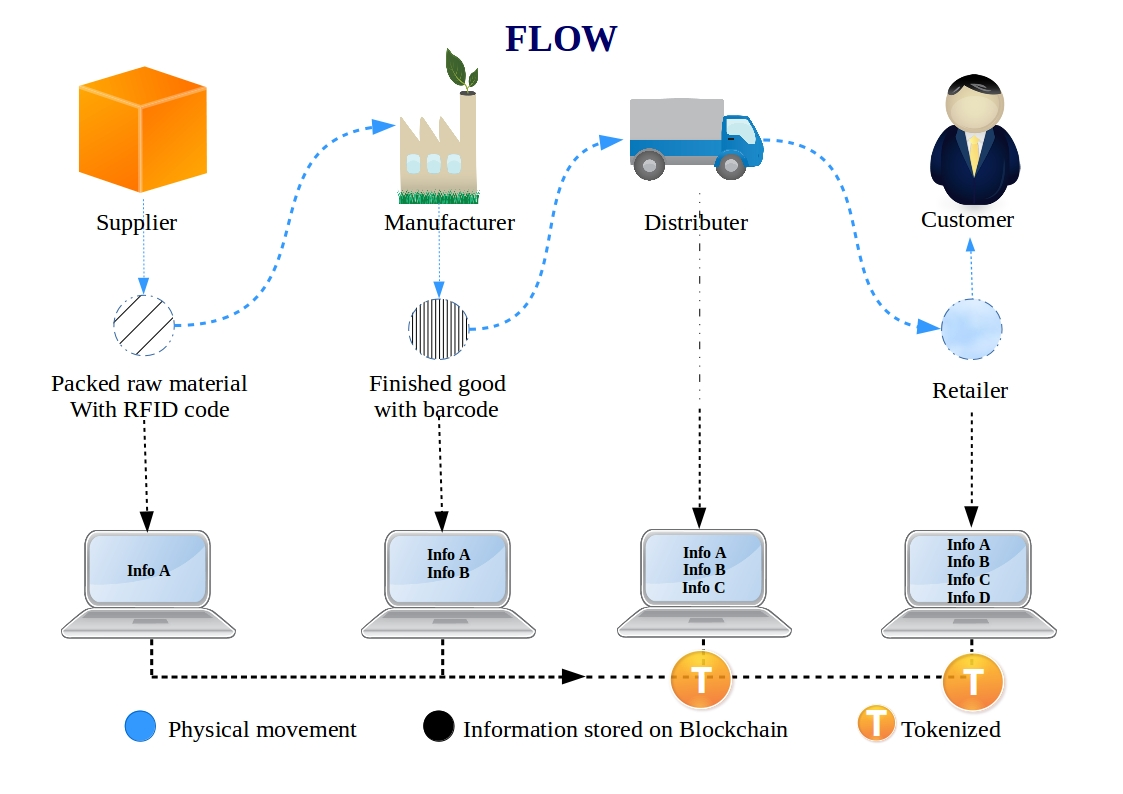
\includegraphics[width=5.99in,height=4.24in]{.//media/1.jpg}
		\caption{Flow Diagram}
	\end{Center}
\end{figure}


%%%%%%%%%%%%%%%%%%%% Figure/Image No: 5 Ends here %%%%%%%%%%%%%%%%%%%%

%Fig 1. Flow Diagram\par

\begin{justify}
{\fontsize{14pt}{16.8pt}\selectfont Different nodes in the system would interact with the blockchain and enter the product detail at that particular time with the use of DApp (Distributed Application). Different IOT sensors or oracles will also capture the data such as humidity, temperature wherever required. The product ownership will be then transfer to different owners throughout the product journey this data will also be stored in the block through smart contract. Consider a sample life cycle of the product A. The Manufacturer order the raw material for the product A. The supplier than packs all the raw material needed along with a RFID code that the supplier will enter this detail in the blockchain and transport it to the manufacturer.\par}
\end{justify}\par

\begin{justify}
{\fontsize{14pt}{16.8pt}\selectfont Manufacturer after receiving the product will confirm the package and enter the necessary details in blockchain. After the product have been Finished a unique number (QRcode, Barcode ,RFID code) would be assigned to the product and product would be tokenized to the Distributor. The distributer after the Transportation of the product will tokenize it to the retailer.\par}
\end{justify}\par

\begin{justify}
{\fontsize{14pt}{16.8pt}\selectfont This system will establish a network of trust through shared ledger, because of neutral participants maintains a permissioned, distributed ledger with copies of authority approval status, full audit history, document filings, and relevant supply chain events, even a small change results in a new immutable block. Cryptography will enable permissioned access only to the participating parties in a particular transaction. All the documentation and authority approvals will be pre-programmed into the blockchain with the help of smart contracts. All filings and approvals of authority can only be changed if approved by the parties taking part in the shipment, This will create trust as\  full audit history is maintained on the Blockchain.\par}
\end{justify}\par


\vspace{\baselineskip}


 %%%%%%%%%%%%  Starting New Page here %%%%%%%%%%%%%%

\newpage

\vspace{\baselineskip}\begin{Center}
\section*{Technology}
\addcontentsline{toc}{section}{Technology}
\end{Center}


%%%%%%%%%%%%%%%%%%%% Figure/Image No: 6 starts here %%%%%%%%%%%%%%%%%%%%

\begin{figure}[H]
	\begin{Center}
		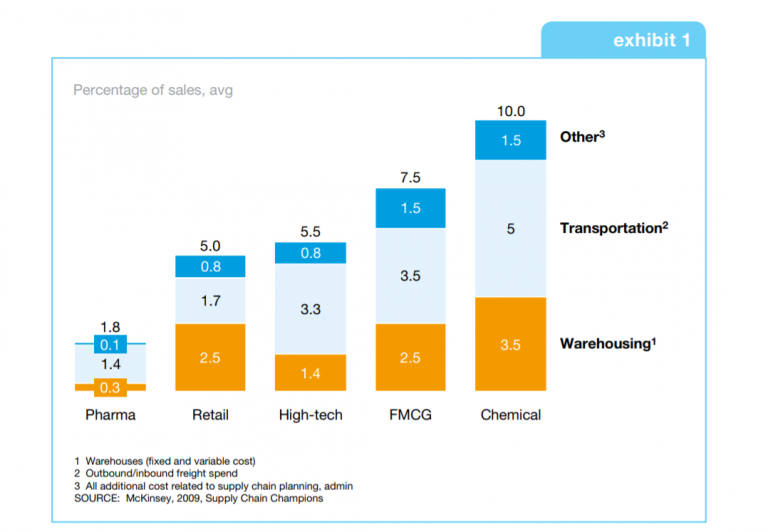
\includegraphics[width=6.01in,height=4.25in]{.//media/2.png}
		\caption{Technology Stack}
	\end{Center}
\end{figure}


%%%%%%%%%%%%%%%%%%%% Figure/Image No: 6 Ends here %%%%%%%%%%%%%%%%%%%%

%Fig 2. Technology Stack\par

{\fontsize{14pt}{16.8pt}\selectfont The above figure shows the technical details of the SCM (Supply chain management) using blockchain. As the system will show information about the transaction to the relevant parties the blockchain network would be permissioned blockchain and we can use the open source blockchain technology such as Hyperledger composer or Corda. We can communicate with other systems through API’s such as REST API. The DApp (Distributed Application) can be web based or Mobile application.\par}\par



 %%%%%%%%%%%%  Starting New Page here %%%%%%%%%%%%%%

\newpage

\vspace{\baselineskip}\begin{Center}
\section*{Analysis}
\addcontentsline{toc}{section}{Analysis}
\end{Center}





%%%%%%%%%%%%%%%%%%%% Figure/Image No: 7 starts here %%%%%%%%%%%%%%%%%%%%

\begin{figure}[H]
	\begin{Center}
		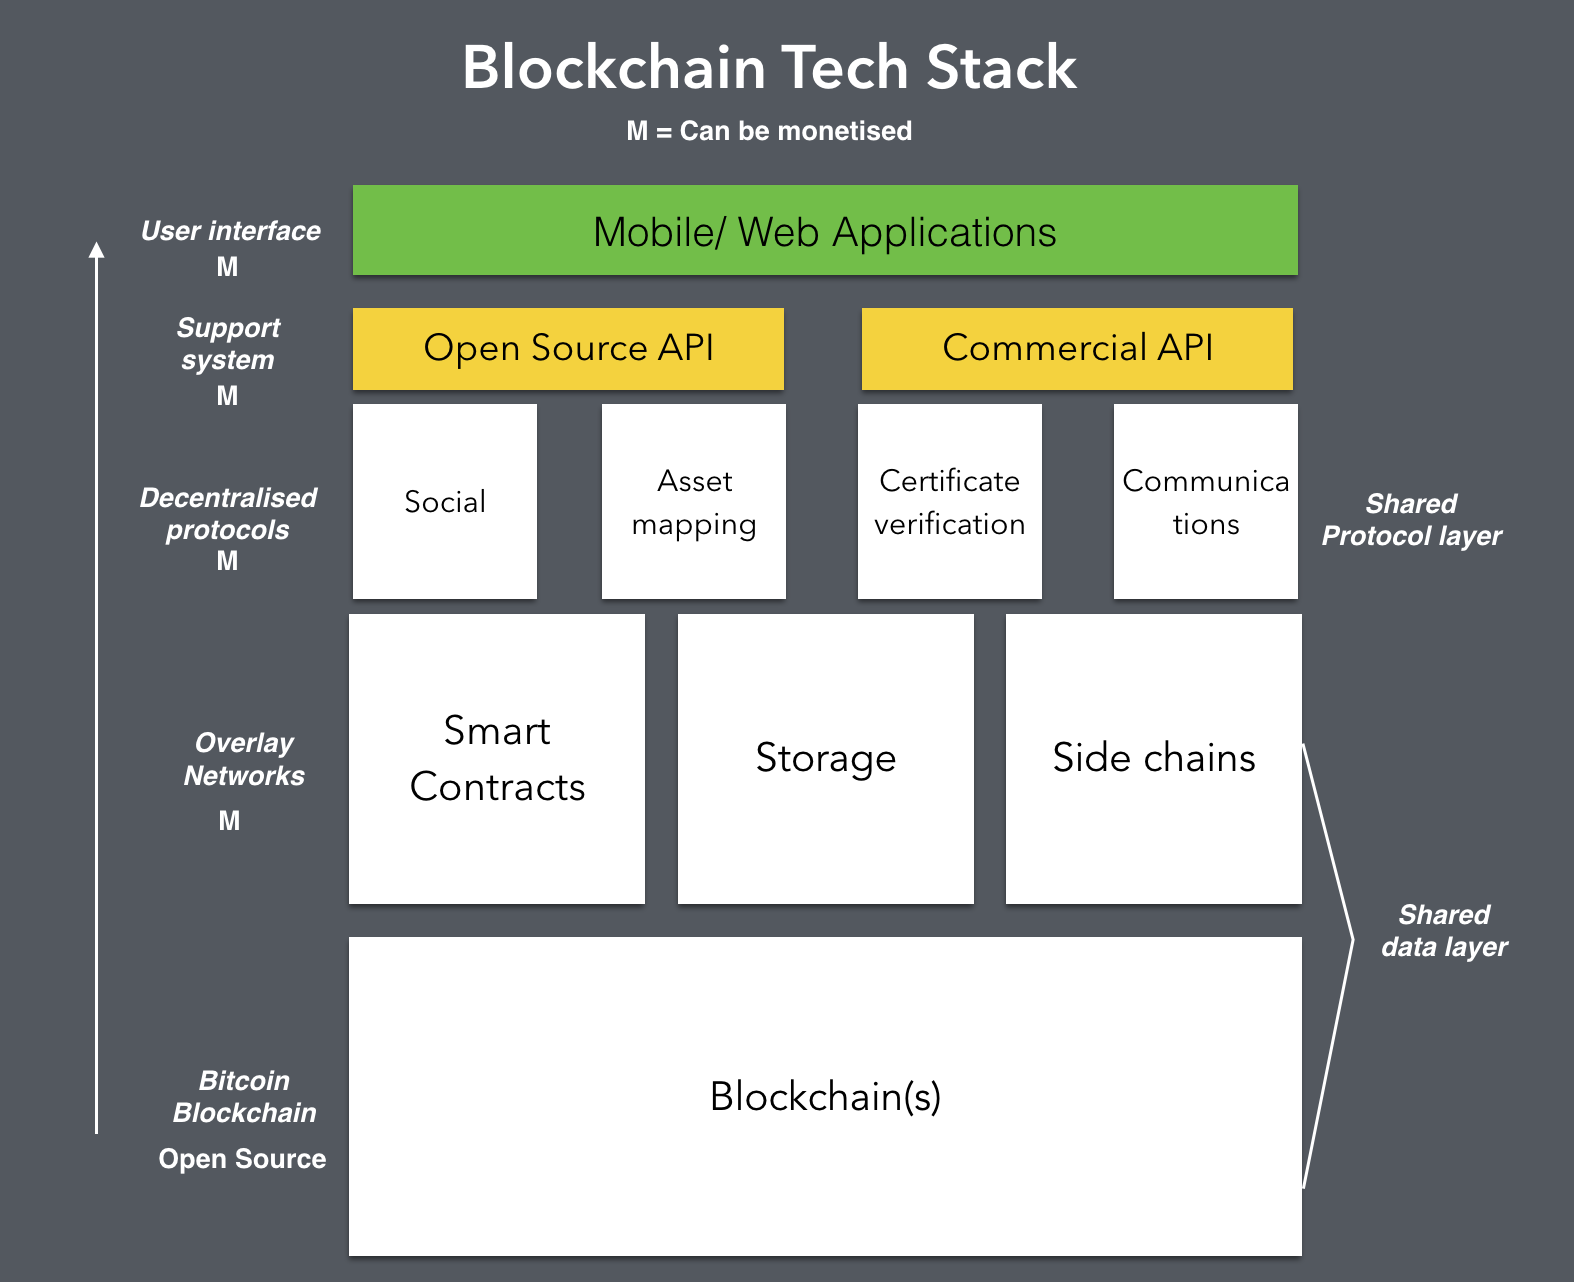
\includegraphics[width=6.01in,height=4.17in]{.//media/3.png}
		\caption{Percentage of Sales}
		\href{https://blog.sv.co/understanding-the-tech-stack-of-blockchain-in-2017-8-years-after-its-launch-48e48f17afea}{Ref.https://blog.sv.co/understanding-the-tech-stack-of-blockchain-in-2017-8-years-after-its-launch-48e48f17afea}
	\end{Center}
\end{figure}

%%%%%%%%%%%%%%%%%%%% Figure/Image No: 7 Ends here %%%%%%%%%%%%%%%%%%%%

%Fig 3. Percentage of Sales\par

{\fontsize{14pt}{16.8pt}\selectfont According to the survey done by McKinsey, $``$Lean and Mean – how does your supply chain shape up?$"$ [9], Most of the cost and time of many supply chain lurks ignored and unmanaged in outbound logistics and behind the closed doors of distribution center. Upto 10$\%$  of overall cost\  of the product is due to supply chain costs, Companies can save 20-50$\%$  in warehousing and up to 40$\%$  in transportation if we can effectively manage the supply chain process.\par}\par


\vspace{\baselineskip}

\vspace{\baselineskip}


 %%%%%%%%%%%%  Starting New Page here %%%%%%%%%%%%%%

\newpage

\vspace{\baselineskip}\begin{Center}
\section*{Conclusion}
\addcontentsline{toc}{section}{Conclusion}
\end{Center}


{\fontsize{14pt}{16.8pt}\selectfont Blockchain is a distributed digital ledger which is immutable. Blockchain build trust in trustless society with the help of technique such as smart contract, cryptography etc. Blockchain is an emerging technology with many application such as supply chain. Blockchain alone is not so effective if we combine it with outer technologies such as RFID, Machine Learning, IoT, etc. will greatly improve the Supply Chain Management process.\par}\par

\begin{justify}
{\fontsize{14pt}{16.8pt}\selectfont Complete transformation of supply chain will not happen in one day, But supply chains can start using blockchain for small portions of the operations. $``$Smart contracts$"$  can play a crucial role to eliminate cost delays and waste currently because of all the paperwork handling done manually. Lastly, Business and brands need to embrace Blockchain technology well in time so that they can reap its reward and get better with time.\par}
\end{justify}\par


\vspace{\baselineskip}

\vspace{\baselineskip}

\vspace{\baselineskip}

\vspace{\baselineskip}

\vspace{\baselineskip}


 %%%%%%%%%%%%  Starting New Page here %%%%%%%%%%%%%%

\newpage

\vspace{\baselineskip}\begin{Center}
\section*{References}
\addcontentsline{toc}{section}{References}
\end{Center}

\begin{enumerate}
	\item  {\fontsize{14pt}{16.8pt}\selectfont Vujicic, Dejan, et al. $``$Blockchain Technology, Bitcoin, and Ethereum: A Brief Overview.$"$  \textit{2018 17th International Symposium INFOTEH-JAHORINA (INFOTEH)}, 2018, doi:10.1109/infoteh.2018.8345547. \par}\par

	\item {\fontsize{14pt}{16.8pt}\selectfont $``$What Is Bitcoin?$"$  \textit{CNNMoney}, Cable News Network, \href{http://money.cnn.com/infographic/technology/what-is-bitcoin/index.html.}{\textcolor[HTML]{1155CC}{money.cnn.com/infographic /technology/what-is-bitcoin/index.html.}}\par}\par

	\item {\fontsize{14pt}{16.8pt}\selectfont Tasatanattakool, Pinyaphat, and Chian Techapanupreeda. $``$Blockchain: Challenges and Applications.$"$  \textit{2018 International Conference on Information Networking (ICOIN)}, 2018, doi:10.1109/icoin.2018.8343163.\par}\par

	\item {\fontsize{14pt}{16.8pt}\selectfont Miller, Dennis. $``$Blockchain and the Internet of Things in the Industrial Sector.$"$  \textit{IT Professional}, vol. 20, no. 3, 2018, pp. 15–18., doi:10.1109/mitp.2018.032501742. \par}\par

	\item {\fontsize{14pt}{16.8pt}\selectfont $``$Lean and Mean-How Does Your Supply Chain Shape Up.$"$  \textit{Scribd}, Scribd, www.scribd.com/document/311191001/Lean-and-Mean-How-Does-Your-Supply-Chain-Shape-Up. \par}\par

	\item {\fontsize{14pt}{16.8pt}\selectfont $``$How Blockchain Revolutionizes Supply Chain Management.$"$  \textit{Digitalist Magazine}, www.digitalistmag.com/finance/2017/08/23/how-the-blockchain-revolutionizes-supply-chain-management-05306209. \par}\par

	\item {\fontsize{14pt}{16.8pt}\selectfont $``$Digitizing Global Trade with Maersk and IBM.$"$  \textit{Blockchain Pulse: IBM Blockchain Blog}, 19 Sept. 2018, \href{http://www.ibm.com/blogs/blockchain/2018/01/digitizing-global-trade-maersk-ibm/}{\textcolor[HTML]{1155CC}{www.ibm.com/blogs/blockchain/2018/01 /digitizing-global-trade-maersk-ibm/}}\par}\par

	\item {\fontsize{14pt}{16.8pt}\selectfont $``$Chain Business Insights Survey Indicates Blockchain Adoption for Supply Chains.$"$  \textit{Allcoinsnews.com}, 29 May 2017, allcoinsnews.com/2017/05/29/chain-business-insights-survey-indicates-blockchain-adoption-for-supply-chains/. \par}\par

	\item {\fontsize{14pt}{16.8pt}\selectfont $``$Blockchain.$"$  \textit{Wikipedia}, Wikimedia Foundation, 14 Mar. 2019, en.wikipedia.org/ wiki/Blockchain$\#$ cite\_note-te20151031-1. \par}\par

	\item {\fontsize{14pt}{16.8pt}\selectfont Wikipedia , $``$Blockchain$"$ , \href{https://en.wikipedia.org/wiki/Blockchain#cite_note-te20151031-1}{\textcolor[HTML]{1155CC}{https://en.wikipedia.org/wiki/Blockchain$\#$ cite\_note-te20151031-1}}\par}\par

	\item {\fontsize{14pt}{16.8pt}\selectfont Bastin, Jacek, et al. $``$Blockchain In: The Supply Chain Industry.$"$  \textit{BitShouts}, 15 Mar. 2019, bitshouts.com/blockchain-supply-chain/. \par}\par

	\item {\fontsize{14pt}{16.8pt}\selectfont Ahram, Tareq, et al. $``$Blockchain Technology Innovations.$"$  \textit{2017 IEEE Technology $\&$  Engineering Management Conference (TEMSCON)}, 2017, doi:10.1109/temscon.2017.799836\par}\par

	\item {\fontsize{14pt}{16.8pt}\selectfont Wikipedia$``$Bitcoin$"$ ,\href{https://en.wikipedia.org/wiki/Bitcoin.}{\textcolor[HTML]{1155CC}{https://en.wikipedia.org/wiki/Bitcoin.}}\par}\par

	\item {\fontsize{14pt}{16.8pt}\selectfont Aziz Muysinaliyev, Sherzod Aktamov , $``$Supply chain management concepts: literature review$"$  , \href{http://www.iosrjournals.org/}{\textcolor[HTML]{1155CC}{www.iosrjournals.org} , Jan. 2014 .}\par}\par

	\item {\fontsize{14pt}{16.8pt}\selectfont Nakamoto S., 2012. $``$Bitcoin: A peer-to-peer electronic cash system$"$ , Oct,2008.\par}\par

	\item {\fontsize{14pt}{16.8pt}\selectfont Morgen Peck , $``$REINFORCING THE LINKS OF THE BLOCKCHAIN$"$ ,IEEE Future Directions BLOCKCHAIN Initiative WHITE PAPER BLOCKCHAININCUBATOR.IEEE.ORG, November 2017 .\par}
\end{enumerate}\par




\newpage

\vspace{\baselineskip}

%%%%%%%%%%%%%%%%%%%% Table No: 7 starts here %%%%%%%%%%%%%%%%%%%%


\begin{table}[H]
 			\centering
\begin{tabular}{p{1in}p{1in}p{1in}p{1in}p{1in}}
\hline
%row no:1
\multicolumn{5}{|p{5in}|}{\Centering {\fontsize{14pt}{16.8pt}\selectfont \textbf{\uline{Seminar Report Documentation}}}} \\
\hline
%row no:2
\multicolumn{3}{|p{3in}}{\textbf{Report Code:}TE-CS-Seminar 2018-2019\tab \tab \tab } & 
\multicolumn{2}{|p{2in}|}{\textbf{Report No:}TCOA-02} \\
\hline
%row no:3
\multicolumn{5}{|p{5in}|}{\textbf{Report Title:} New\ \ Approach\ \ to\ \ SCM  (Supply Chain Management)  using  Blockchain } \\
\hhline{--}
%row no:4
\multicolumn{5}{|p{5in}|}{\textbf{Address:}Dr. D. Y. Patil Institute of Technology, Sant Tukaram Nagar, Pimpri, Pune, Pin-411018, M.S.India.  } \\
\hline
%row no:5
\multicolumn{5}{|p{5in}|}{\textbf{Address:} Sant Tukaram Nagar,Pimpri, Pune-411018. \par \textbf{E-mail:\href{mailto:ayushbansal323@gmail.com}{ ayushbansal323@gmail.com}} \par \textbf{Cell-no:} 7776075075 } \\
\hline
%row no:6
\multicolumn{5}{|p{5in}|}{\textbf{Year:} 2018-2019 \par \textbf{Branch:} Computer Engineering  } \\
\hline
%row no:7
\multicolumn{5}{|p{5in}|}{\textbf{Keywords:}{\fontsize{14pt}{16.8pt}\selectfont \ Blockchain, SCM (Supply Chain Management), Bitcoin , Smart Contract, RFID, Token, Node.} } \\
\hline
%row no:8
\multicolumn{1}{|p{1in}}{\textbf{Type    of Report:} Final} & 
\multicolumn{1}{|p{1in}}{\textbf{Report checked By:}} & 
\multicolumn{1}{|p{1in}}{\textbf{Report checked Date:}} & 
\multicolumn{1}{|p{1in}}{\textbf{Guide’s complete Name:} Prof. Latika Desia \vspace{\baselineskip}\vspace{\baselineskip}} & 
\multicolumn{1}{|p{1in}|}{{\fontsize{14pt}{16.8pt}\selectfont \textbf{Total copies:} 2}} \\
\hline
\end{tabular}
 \end{table}


%%%%%%%%%%%%%%%%%%%% Table No: 7 ends here %%%%%%%%%%%%%%%%%%%%


\vspace{\baselineskip}


\end{document}
